\section{Theorie}

\subsection{Was ist ein Raytracer?}

Dazu muss zu Erst der Begriff \textit{Rendering} erklärt werden. Dieser beschreibt ganz Allgemein den Prozess, der aus der Beschreibung einer dreidimensionalen Szene ein zweidimensionales Bild erzeugt. Dazu sind zahlreiche Algorithmen notwendig, welche beispielsweise Geometrien modellieren, Objekte animieren oder Texturen erzeugen und die Ergebnisse hiervon an den Render-Prozess weitergeben, um diese sichtbar zu machen. 

Um eine dreidimensionale Szene in ein Bild abzubilden, kann sich des Ray-tracing Algorithmuses bedient werden. Wie sich bereits aus dem Begriff ableiten lässt, werden dabei die Pfade einzelner "`Lichtstrahlen"' verfolgt, bis diese auf eine Oberflächen treffen und es beispielsweise zu einer Reflektion kommt. 

Da dabei nur diejenigen Strahlen von Interesse sind, welche auch tatsächlich auf den virtuellen Bildsensor treffen und auf ein Pixel im Bild abgebildet werden, verfolgen Ray-tracer diese in umgekehrter Richtung. Es werden also Strahlen am Bildsensor erzeugt und in die Szene geschickt. Auf diese Weise werden alle Lichtquellen identifiziert, die einen Beitrag zum Helligkeits- und Farbwert des gerade betrachteten Pixels leisten \cite{pbrt_book}. 

Der in dieser Arbeit genutzte Ray-tracer ist \textit{pbrt}\cite{pbrt}. Dieser hat den Anspruch das Rendering \textit{physically based}, also möglichst physikalisch korrekt, durchzuführen. Aus diesem Grund sind hier viele grundlegenden Gleichungen der Optik implementiert und Phänomene werden so korrekt berechnet. Im Gegensatz dazu stehen Ray-tracer, welche für Animationsfilme oder Computerspiele genutzt werden. Hier soll das Endergebnis möglichst \textit{gut} aussehen, ohne unbedingt physikalisch korrekt zu sein. 

Trotz des Anspruchs von \textit{pbrt} möglichst physikalisch korrekte Resultate zu erzeugen, sind manche optische Phänomene noch nicht implementiert. So besteht im Moment noch keine Möglichkeit die optischen Verzerrungen nachzubilden, welche von allen realen Optiken verursachet werden.

In der vorliegenden Arbeit soll ein neues Kameramodell in den frei verfügbaren Quellcode von \textit{pbrt} eingefügt werden, welches gemessenen Verzerrungen von Optiken berechnet.

\subsection{Verzerrung}

Die Verzerrungen, welche von realen Optiken verursacht werden, führen dazu, dass in der Realität ungekrümmte Linien in der zweidimensionalen Abbildung gekrümmt erscheinen. Dies geschieht dadurch, dass Punkte im aufgenommenen Bild verschoben erscheinen und zwar umso stärker, je weiter sie von der optischen Achse entfernt sind. Besondern gut lässt sich dieser Effekt bei weitwinkligen Objektiven an Hausfassaden beobachten. 

Genauer wird dabei zwischen Tonnen- und Kissenverzeichnung unterschieden. In Abbildung \ref{fig:distortionBarrel} und \ref{fig:distortionPinc} wird deutlich, dass im ersten Fall die Bildpunkte von der optischen Achse weg verschoben werden, während der Abstand der Bildpunkte zur optischen Achse bei der Tonnenverzeichnung kleiner wird. Durch die bereits erwähnte Zunahme dieses Effekts mit steigendem Radius zur optischen Achse, erfahren eigentlich gerade Linien eine Krümmung \cite{smith2000modern}.

\begin{figure}[h]
	\begin{minipage}{.5\textwidth}
		\centering
		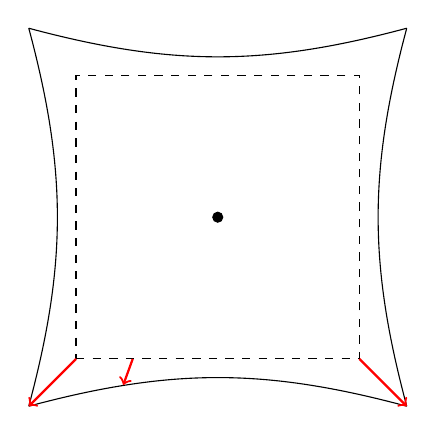
\begin{tikzpicture}[scale=0.6]
		% undistorted:
		\draw[black, dashed] (-3, -3) -- (3, -3) -- (3, 3) -- (-3, 3) -- (-3, -3);
		
		% distorted pincushion
		\draw (-4 ,-4) to[out=15,in=165] (4 , -4);
		\draw (4 ,-4) to[out=105,in=255] (4 , 4);
		\draw (4 ,4) to[out=195,in=-15] (-4 , 4);
		\draw (-4 ,4) to[out=285,in=75] (-4 , -4);
		
		% optical centre
		\filldraw 
		(0,0) circle (3pt);
		
		%distortion arrows
		\draw [red, ->, thick] (-3, -3) -- (-4, -4);
		\draw [red, ->, thick] (3, -3) -- (4, -4);
		\draw [red, ->, thick] (-1.8, -3) -- (-2., -3.55);
		
		\end{tikzpicture}
		\caption{Kissenverzeichnung}
		\label{fig:distortionBarrel}
	\end{minipage}
	\begin{minipage}{.5\textwidth}
		\centering
		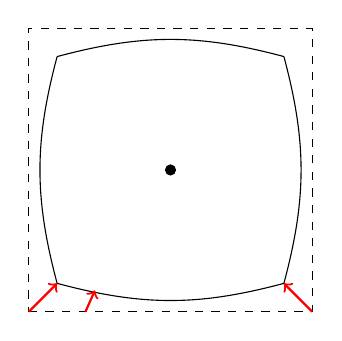
\begin{tikzpicture}[scale=0.6]
		% undistorted
		\draw[black, dashed] (-3, -3) -- (3, -3) -- (3, 3) -- (-3, 3) -- (-3, -3);
		
		%distorted barrel
		
		\draw (-2.4 ,-2.4) to[out=-15,in=-165] (2.4 , -2.4);
		\draw (2.4 ,-2.4) to[out=75,in=285] (2.4 , 2.4);
		\draw (2.4 ,2.4) to[out=165,in=15] (-2.4 , 2.4);
		\draw (-2.4 ,2.4) to[out=255,in=105] (-2.4, -2.4);
		
		% optical centre
		\filldraw 
		(0,0) circle (3pt);
		
		%distortion arrows
		\draw [red, ->, thick] (-3, -3) -- (-2.4, -2.4);
		\draw [red, ->, thick] (3, -3) -- (2.4, -2.4);
		\draw [red, ->, thick] (-1.8, -3) -- (-1.6, -2.55);
 	     
	    		
		\end{tikzpicture}
		\caption{Tonnenverzeichnung}
		\label{fig:distortionPinc}
	\end{minipage}
	
\end{figure}

\subsection{Lochkameramodell}

\begin{figure}[h]
	\centering
	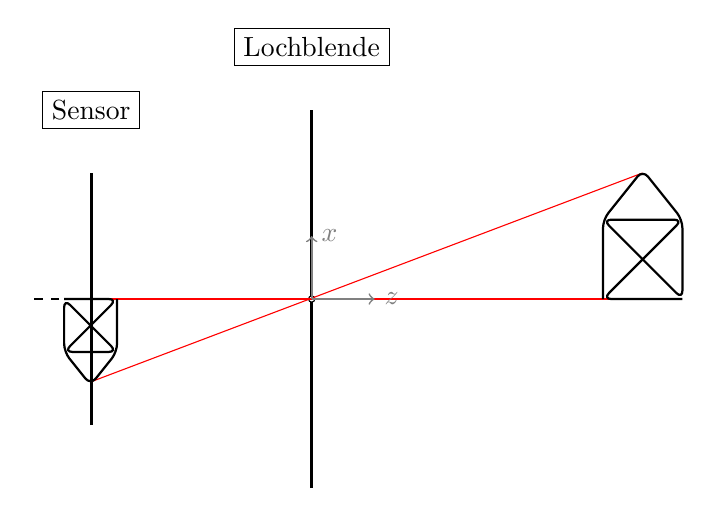
\begin{tikzpicture}[scale=0.4]
	
	% sensor
	\draw[very thick] (-7,-4) -- (-7, 4);
	% lochblende
	\draw (0,0) circle [radius=0.1];
	\draw[very thick] (0, -6) -- (0, -0.1);
	\draw[very thick] (0, 6) -- (0, 0.1);
	%optische Achse
	\draw[thin, dashed] (2, 0) -- (-9, 0);
	%Lichtstrahl Dach
	\draw[red] (10.5, 4) -- (-7, -21/8);
	%Lichtstrahl Boden
	\draw[red] (10.5, 0) -- (-7, 0);
	%Koordinatensystem
	\draw[semithick, gray, ->] (0,0) -- (0,2) node[right] {$x$};
	\draw[semithick, gray, ->] (0,0) -- (2,0) node[right] {$z$};
	%Beschriftung
	\node[draw] at (-7, 6) {Sensor};
	\node[draw] at (0, 8) {Lochblende};
	
	% Nikolaus echt
	 \begin{scope}[shift={(9.25,0)}, scale=1.26]
	\draw[thick,rounded corners=3pt] (0,0) -- (0,2) -- (1,3.25) 
	-- (2,2) -- (2,0) -- (0,2) -- (2,2) -- (0,0) -- (2,0);
	\end{scope}
	
	% Nikolaus Abbildung
	\begin{scope}[shift={(-6.18,0)}, scale=0.84, rotate=180]
	\draw[thick,rounded corners=3pt] (0,0) -- (0,2) -- (1,3.25) 
	-- (2,2) -- (2,0) -- (0,2) -- (2,2) -- (0,0) -- (2,0);
	\end{scope}
	
	\end{tikzpicture}
	\caption{Lochkamera}
	\label{fig:pinholeCam}
\end{figure}

\subsection{Verzerrungsmodelle}

\subsection{Integrations der Verzerrung in den Raytracer}

%\subsubsection{Konzept ( Warum muss man invertieren? )}

%Das Lochkamera-Modell geht von einer infinitesimal kleinen Blendenöffnung aus. Einfallende Lichtstrahlen, die auf die Öffnung treffen, bewegen sich ungehindert in ihre Ausbreitungsrichtung weiter und treffen an einem Punkt $p_1$ auf den Kamerasensor (siehe blauer Strahl in Abbildung \ref{fig:model}).
Die Auswirkungen einer Linsenverzerrung sind in Abbildung \ref{fig:model} dargestellt. Der Lichtstrahl bewegt sich nicht mehr ungehindert in seiner Ausbreitungsrichtung weiter und trifft an einem Punkt $p_1$ auf den Kamerasensor (siehe blauer Strahl), sondern
wird an der Öffnung der Lochblende in einem bestimmten Maße abgeknickt und erreicht den Sensor am Punkt $p_2$ (roter Strahl). Die Funktion, die die normalisierten Pixelkoordinaten des unverzerrten Punktes $p_1$ auf die des verzerrten Punktes $p_2$ abbildet, bezeichnen wir mit $f$.
\begin{figure}[h]
	\centering
	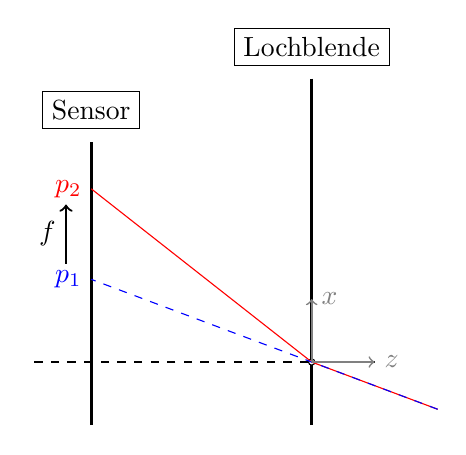
\begin{tikzpicture}[scale=0.4]

	% sensor
	\draw[very thick] (-7,-2) -- (-7, 7);
	% lochblende
	\draw (0,0) circle [radius=0.1];
	\draw[very thick] (0, -2) -- (0, -0.1);
	\draw[very thick] (0, 9) -- (0, 0.1);
	%optische Achse
	\draw[thin, dashed] (2, 0) -- (-9, 0);
	%abgelenkter Lichtstrahl
	\draw[red] (4, -1.5) -- (0, 0) -- (-7, 5.5) node[left] {$p_2$};
	%durchgehender Lichtstrahl
	\draw[blue, dashed] (4, -1.5) -- (-7, 21/8) node[left] {$p_1$};
	%Verzeichnungspfeil
	\draw[->, thick] (-7.8, 21/8 + 0.5) -- (-7.8, 65/16) node[left] {$f$} -- (-7.8, 5) ;
	%Koordinatensystem
	\draw[semithick, gray, ->] (0,0) -- (0,2) node[right] {$x$};
	\draw[semithick, gray, ->] (0,0) -- (2,0) node[right] {$z$};
	%Beschriftung
	\node[draw] at (-7, 8) {Sensor};
	\node[draw] at (0, 10) {Lochblende};
	\end{tikzpicture}
	\caption{Vereinfachtes Verzerrungsmodell in 2D. Der rote von rechts einfallende Lichtstrahl wird durch die Linse abgelenkt. In blau ist der Weg dargestellt, den der Strahl nach dem Lochkamera-Modell nehmen würde. Die gestrichelte Linie zeigt die optische Achse. Die Abbildung zwischen Lochkamera-Modell und Modell mit Verzerrung ist mit $f$ bezeichnet.}
	\label{fig:model}
\end{figure}
Ein Raytracer, der eine solche Linsenverzerrung berücksichtigen soll, muss also bei der Erzeugung der Strahlen für einen gegebenen Punkt von dem Lochkamera-Modell aus Abschnitt \ref{sec:pinhole} abweichen.

 Allerdings gibt es für jeden Punkt $p$ auf dem Sensor einen Punkt $p'$, deren zugeordneter Strahl für $z\ge0$ \emph{nach dem Lochkamera-Modell} dem Strahl entspricht, der \emph{nach dem Verzerrungsmodell} $p$ zuzuordnen ist.
In Abbildung \ref{fig:model} ist $p = p_2$ und $p' = p_1$. Da $f(p_1) = p_2$ ist, kann damit $p'$ durch Anwenden der inversen Verzerrungsfunktion $g = f^{-1}$ mit $p' = g(p)$ gefunden werden. Der Strahl für $p$ kann dann einfach nach dem Lochkamera-Modell berechnet werden, indem $p = p'$ gesetzt wird.
